\newpage
\section{Mechanical Specifications}
\label{sec:Mechanical}

\hspace*{0.5cm}
\begin{minipage}{\linewidth-0.5cm}
  \begin{enumerate}[label=\Alph*.]
    
  \item Measured weight of the payload (not including payload plate): \newline
        The estimated weight is \SI{1700}{\gram}. The final weight will be measured once all components have arrived.
    
  \item The following mechanical drawings and pictures of the SORA components illustrate how our payload is attached to the payload mounting plate. All dimensions are in \textbf{metric units}.
    
  \item This is not a pressurized vessel. The collection containers illustrated in Figure 5 will receive air from the actuator-pump system. However, there are pressure release valves to prevent the Clean Box from becoming a pressurized vessel. Therefore, there should not be anything potentially hazardous to the ground crew before or after launch.

  \item No other mechanical information at this time.

  \end{enumerate}
\end{minipage}


\begin{centering}
  \begin{figure}[h]
    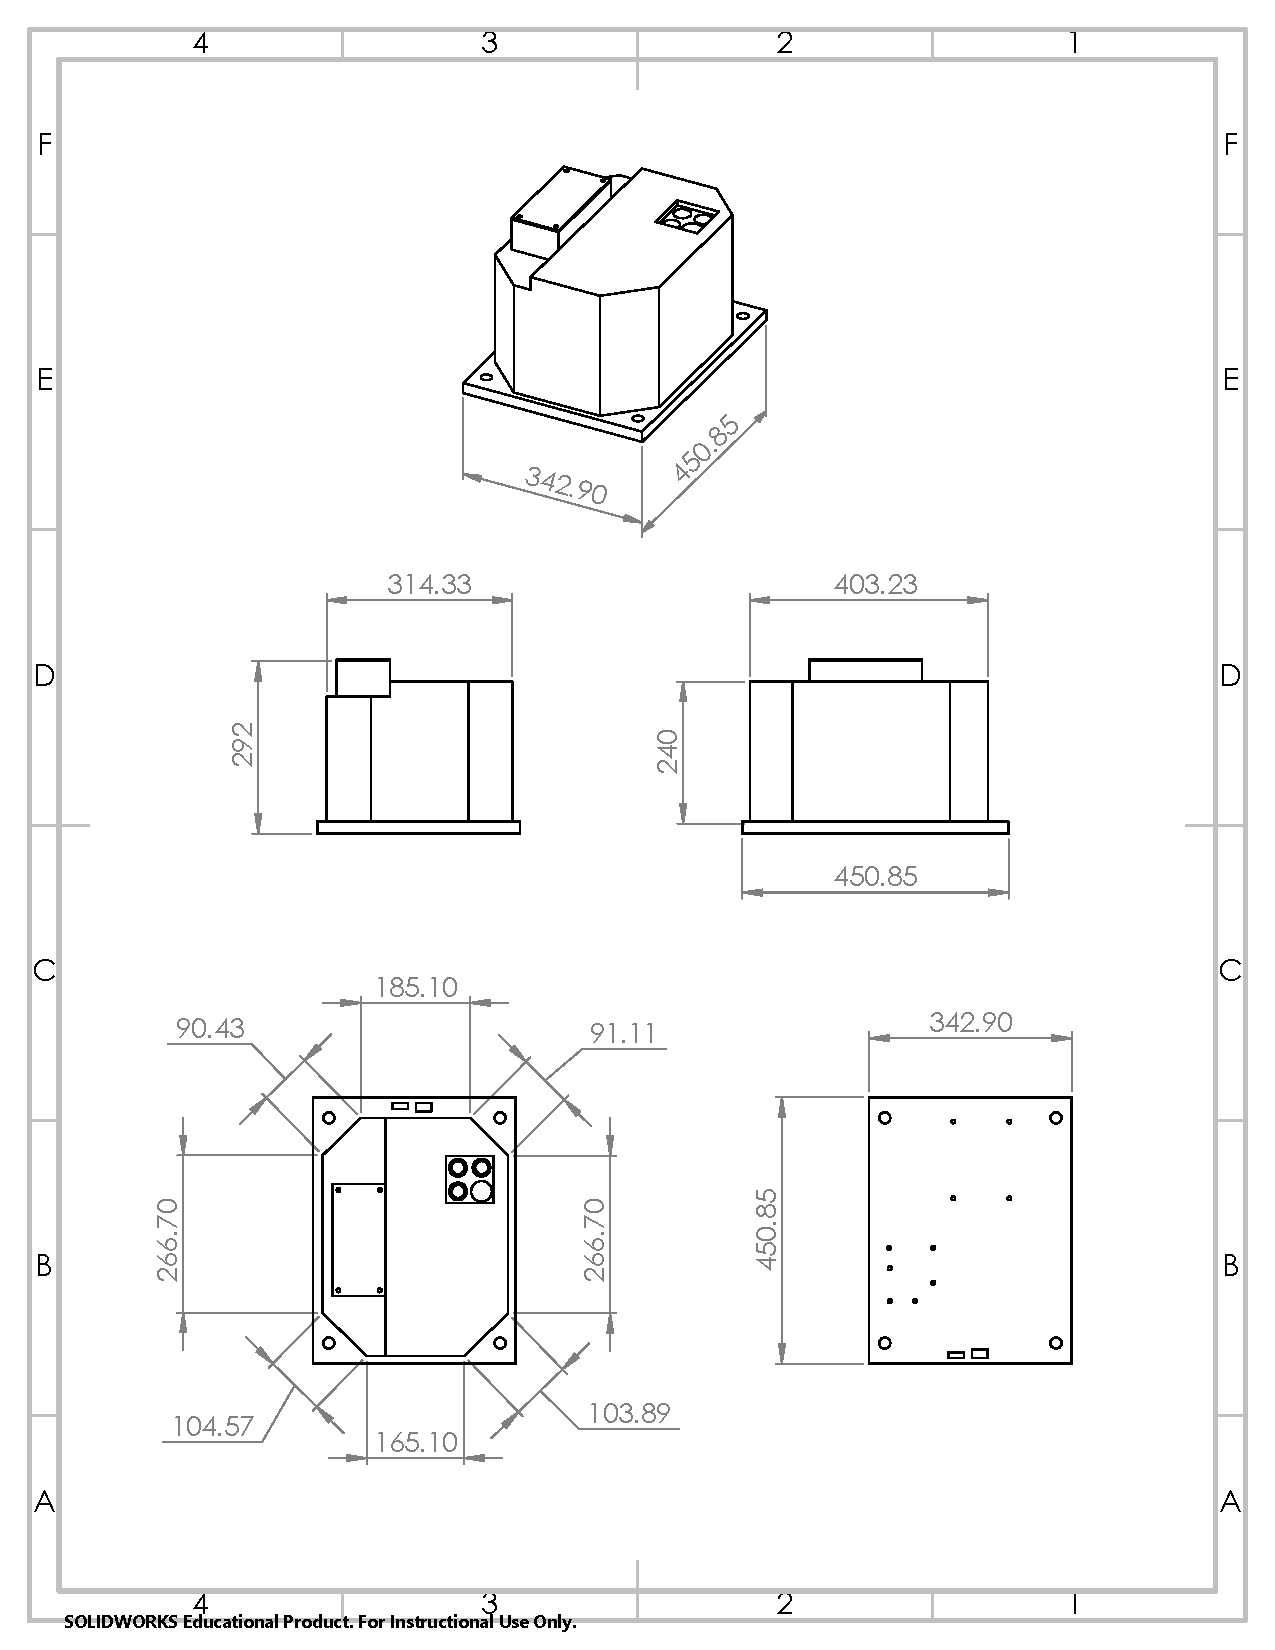
\includegraphics[width=0.9\textwidth]{Figures/payload_plate.pdf}
    \caption{Updated desgin with new collection system (all in millimeters).}
    \label{fig:PayloadPlate}
  \end{figure}

  \newpage
  
  \begin{figure}[h]
    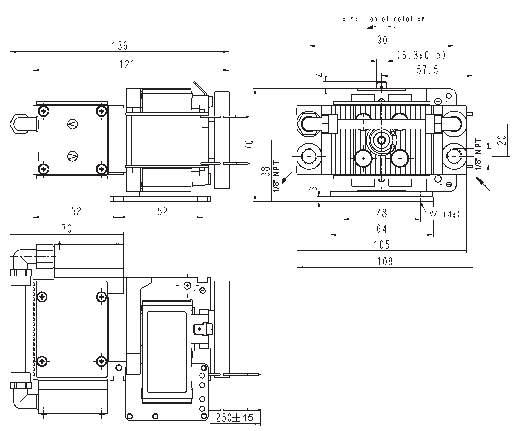
\includegraphics[width=\textwidth]{Figures/pumps.pdf}
    \caption{Pumps (all in millimeters).}
    \label{fig:Pumps}
  \end{figure}
  
  \newpage
  
  \begin{figure}[h]
    \includegraphics[width=\textwidth]{Figures/pump_mounts.pdf}
    \caption{Pump mounts (all in millimeters).}
    \label{fig:PumpMounts}
  \end{figure}
  
  \newpage
  
  \begin{figure}[h]
    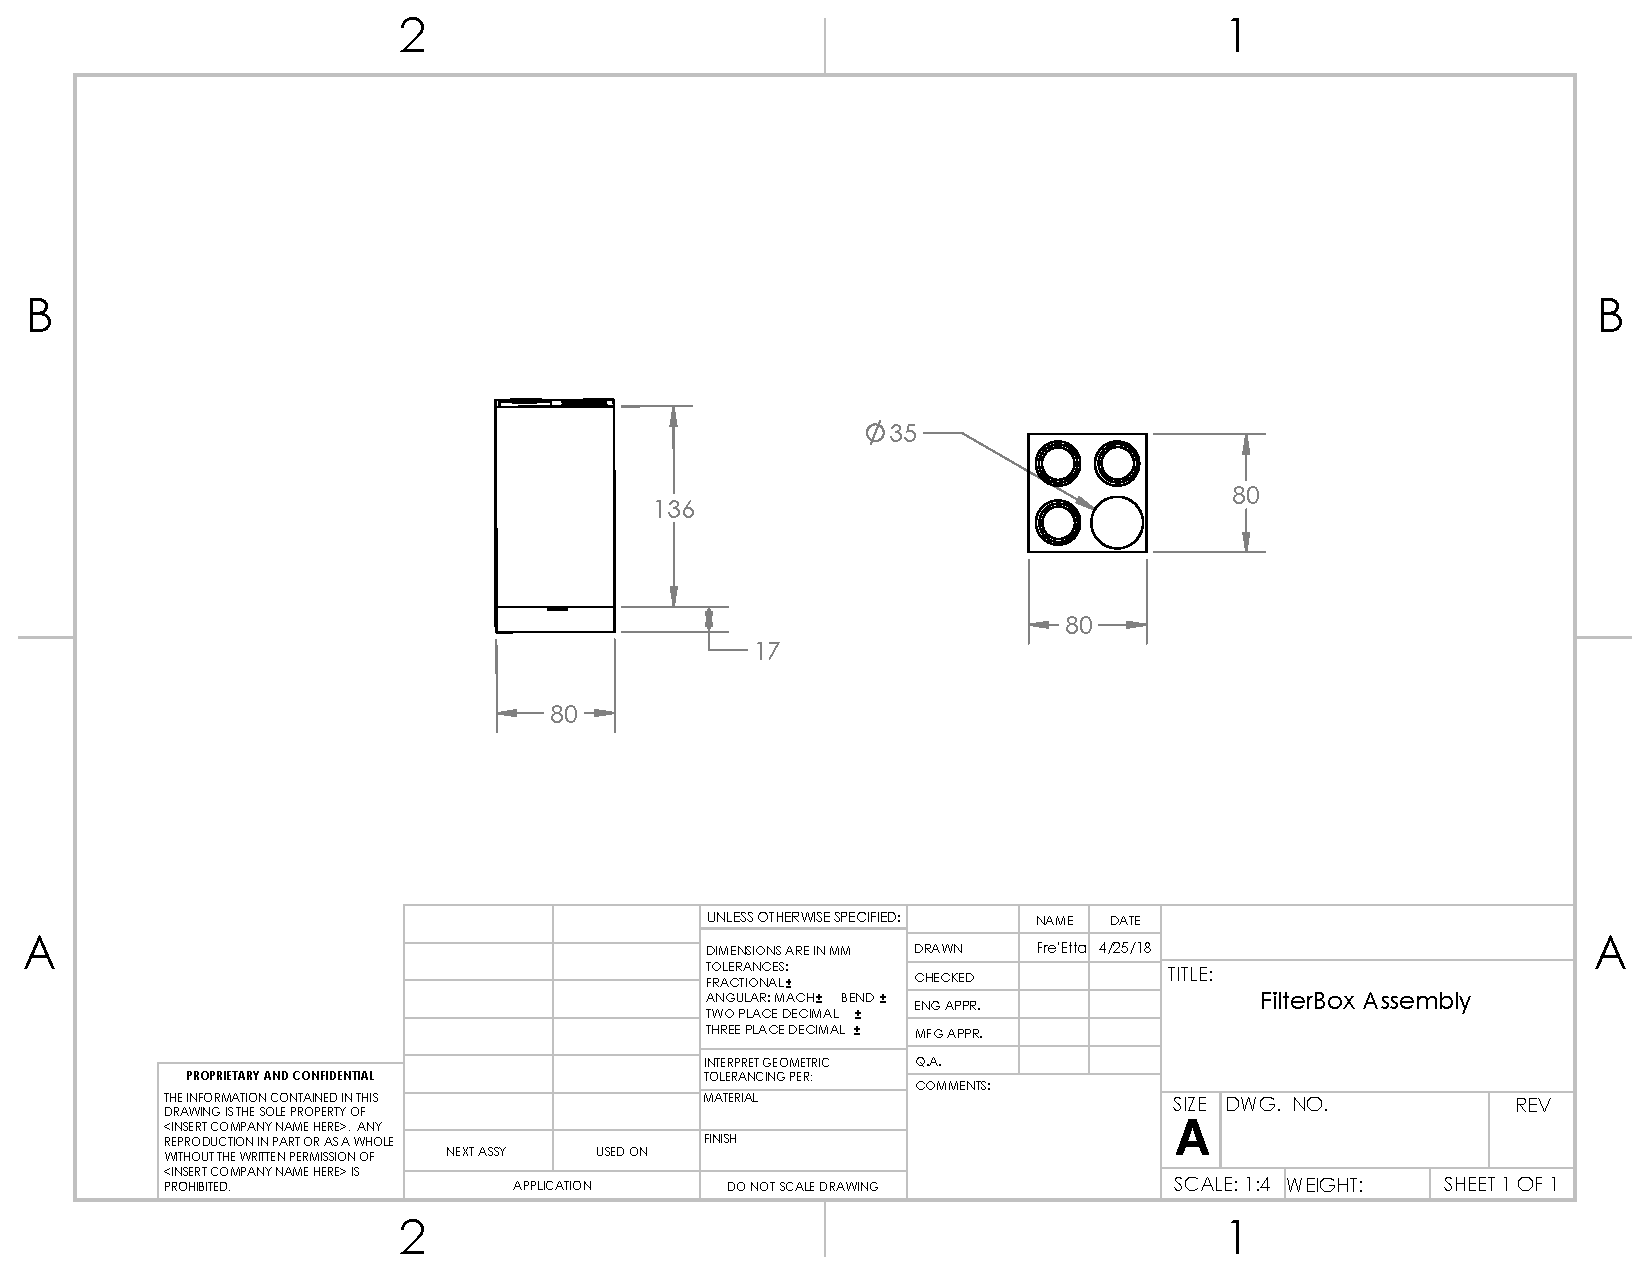
\includegraphics[width=\textwidth]{Figures/filter_box_assembly.pdf}
    \caption{Passive clean box (all in millimeters).}
    \label{fig:FilterBox}
  \end{figure}
  
  \newpage
  
  \begin{figure}[h]
    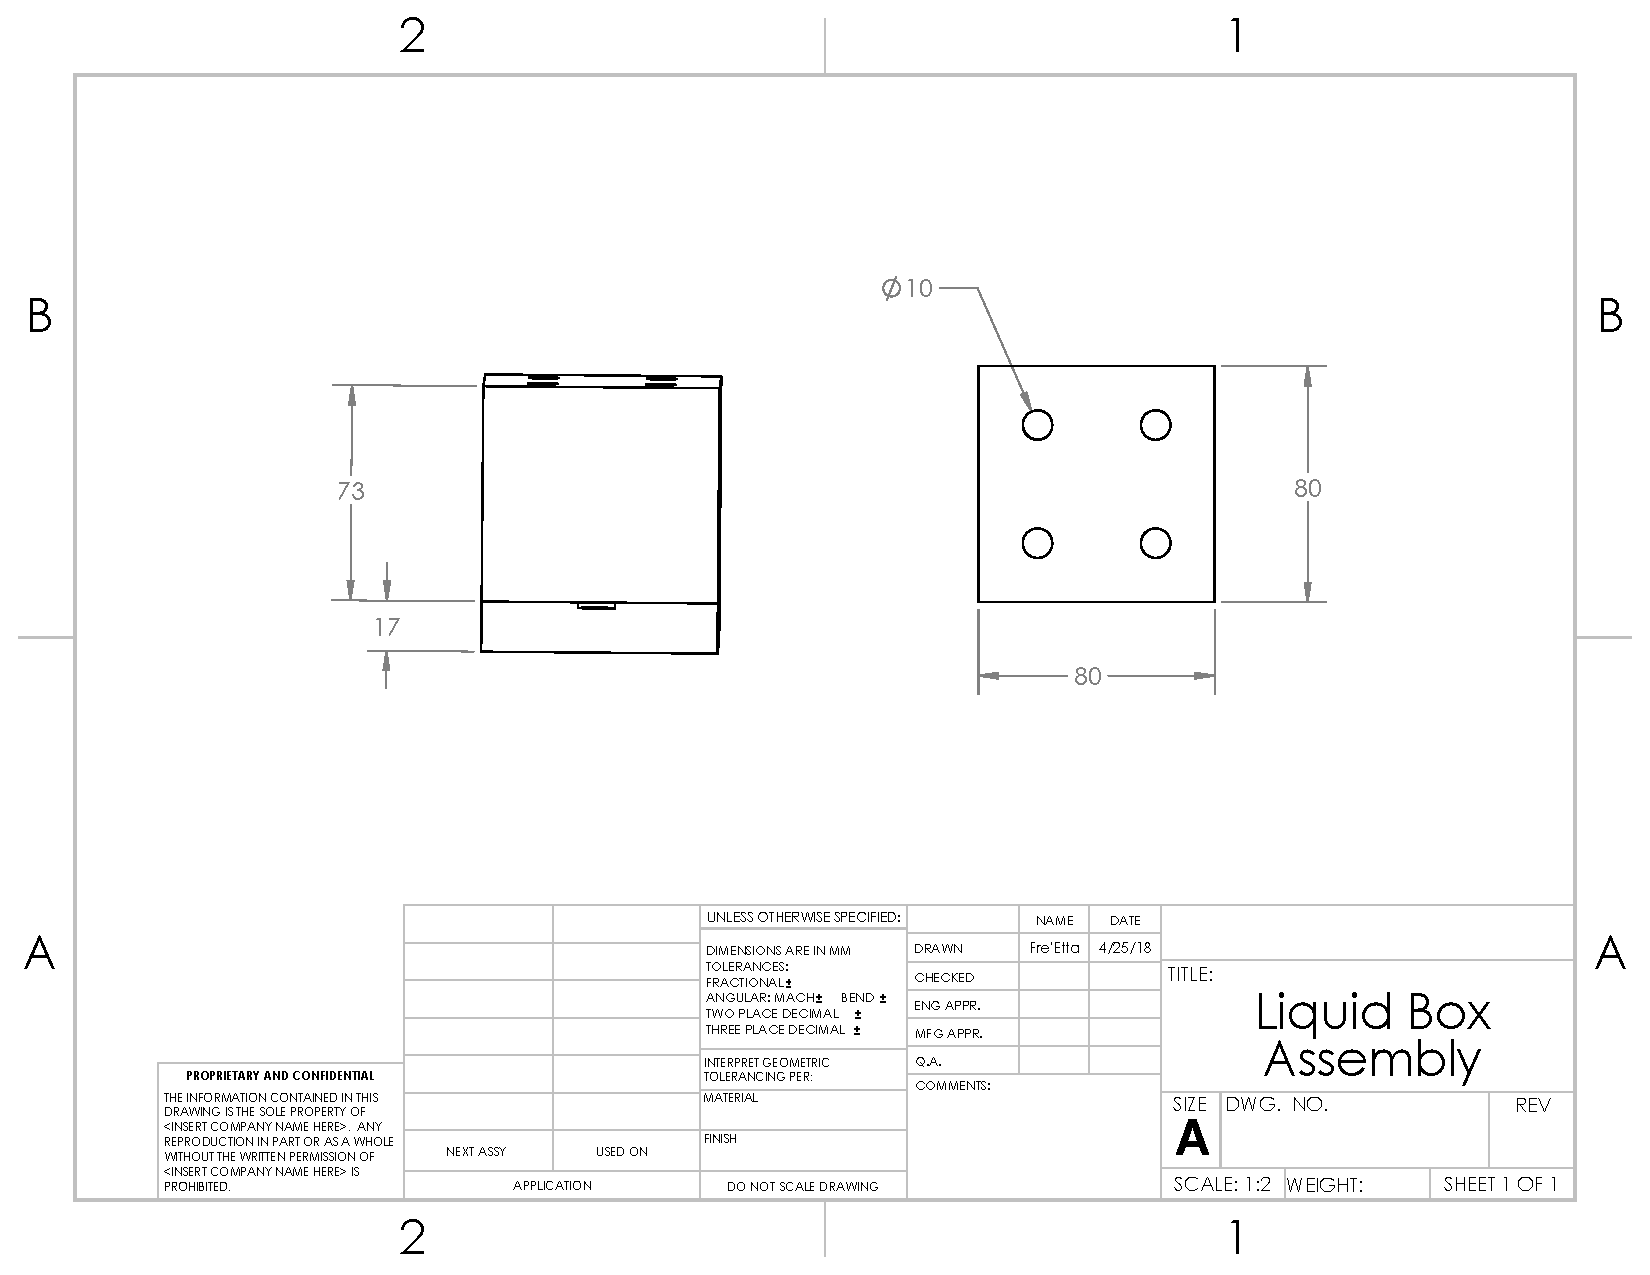
\includegraphics[width=\textwidth]{Figures/liquid_box_assembly.pdf}
    \caption{Liquid clean box (all in millimeters).}
    \label{fig:LiquidBox}
  \end{figure}
  
  \newpage
  
  \begin{figure}[h]
    \includegraphics[width=\textwidth]{Figures/electronics_box.pdf}
    \caption{See through electronics box (all in millimeters).}
    \label{fig:ElectronicsBox}
  \end{figure}
\end{centering}
